\begin{comment}
\section{Dataset, relevantná literatúra, prehľad existujúcich riešení}

The dataset provided for this challenge consists of 7 546 different food recall announcements. However, for the purpose of the challenge submissions were only evaluated on reports that were in the English language, of which there are 6 644 \cite{randl-etal-2025-semeval, randl_2025_15007331}. The remaining reports in different languages, of which there are 902, were only added to the dataset as supplementary training data. The final version of the dataset used in the challenge is publicly available on Zenodo \cite{randl_2025_15007331}. 

These reports were scraped from 24 official government food authorities (mostly based in the US, the UK, Canada and Australia) and labeled by experts with the help of the company Agroknow \cite{randl_2025_15007331}. The dataset provides 6 input features:

\begin{itemize}
    \item \textit{title} - the title of the announcement
    \item \textit{text} - raw text body of the announcement 
    \item \textit{country} - country of issue
    \item \textit{year} - year when the report was published
    \item \textit{month} - month when the report was published
    \item \textit{day} - day when the report was published
\end{itemize}

As can be seen in the official report the majority of submissions only used the \textit{title} and \textit{text} features (or just \textit{title} or \textit{text}) with only 3 out of 27 teams choosing to include all provided features \cite{randl-etal-2025-semeval}.

For target features there are the aforementioned categorical and specific features:

\begin{itemize}
    \item \textit{product-category} -- category of product, 22 provided labels, used for sub-task 1
    \item \textit{hazard-category} -- category of hazard, 10 provided labels, used for sub-task 1
    \item \textit{product} -- specific product, 1 142 provided labels, used for sub-task 2
    \item \textit{hazard} -- specific hazard, 128 provided labels, used for sub-task 2
\end{itemize}

A notable feature that makes this challenge hard is the heavy class imbalance of the dataset, every target feature has a long-tailed label distribution, with many rare classes (see Figure~\ref{fig:placeholder}) \cite{randl-etal-2025-semeval}. All 4 of the top-scoring solutions highlighted in the report chose to tackle this problem directly by the use of data augmentation \cite{zhang-etal-2025-srcb, le-etal-2025-anastasia, phan-chiang-2025-mymy, wan-etal-2025-pateam}.
\end{comment}

\section{Dataset, relevantná literatúra, prehľad existujúcich riešení}

Dataset poskytnutý pre túto súťaž obsahuje 7\,546 oznámení o sťahovaní potravín z trhu. Riešenia v súťaži však boli hodnotené iba na správach v anglickom jazyku, ktorých je 6\,644 \cite{randl-etal-2025-semeval, randl_2025_15007331}. Zvyšných 902 správ v iných jazykoch bolo do datasetu pridaných iba ako doplnkové trénovacie dáta. Finálna verzia datasetu použitá v súťaži je verejne dostupná na platforme Zenodo \cite{randl_2025_15007331}.

Správy boli získané z webových stránok 24 oficiálnych vládnych potravinových úradov (najmä v USA, Spojenom kráľovstve, Kanade a Austrálii) a anotované expertmi v spolupráci so spoločnosťou Agroknow \cite{randl_2025_15007331}. Dataset poskytuje 6 vstupných atribútov:

\begin{itemize}
    \item \textit{title} -- názov oznámenia,
    \item \textit{text} -- neupravený text oznámenia,
    \item \textit{country} -- krajina vydania,
    \item \textit{year} -- rok zverejnenia správy,
    \item \textit{month} -- mesiac zverejnenia správy,
    \item \textit{day} -- deň zverejnenia správy.
\end{itemize}

Ako uvádza oficiálny článok, väčšina riešení využívala iba atribúty \textit{title} a \textit{text} (prípadne iba jeden z nich) a len 3 z 27 tímov sa rozhodli použiť všetky dostupné atribúty \cite{randl-etal-2025-semeval}.

Cieľovými atribútmi sú vyššie spomínané kategórie a konkrétne označenia:

\begin{itemize}
    \item \textit{product-category} -- kategória produktu, 22 labelov, použitá v podúlohe 1,
    \item \textit{hazard-category} -- kategória hazardu, 10 labelov, použitá v podúlohe 1,
    \item \textit{product} -- konkrétny produkt, 1\,142 labelov, použitý v podúlohe 2,
    \item \textit{hazard} -- konkrétny hazard, 128 labelov, použité v podúlohe 2.
\end{itemize}

Výraznou vlastnosťou, ktorá túto súťaž sťažuje, je silná nevyváženosť tried v datasete. Každý cieľový atribút má rozdelenie labelov s dlhým chvostom (long-tailed distribution), teda s množstvom zriedkavých tried (viď obrázok~\ref{fig:dataset_distribution}) \cite{randl-etal-2025-semeval}. Všetky 4 najlepšie riešenia opísané v oficiálnom článku sa tento problém rozhodli riešiť priamo, pomocou augmentácie dát \cite{zhang-etal-2025-srcb, le-etal-2025-anastasia, phan-chiang-2025-mymy, wan-etal-2025-pateam}.

\begin{figure}
    \centering
    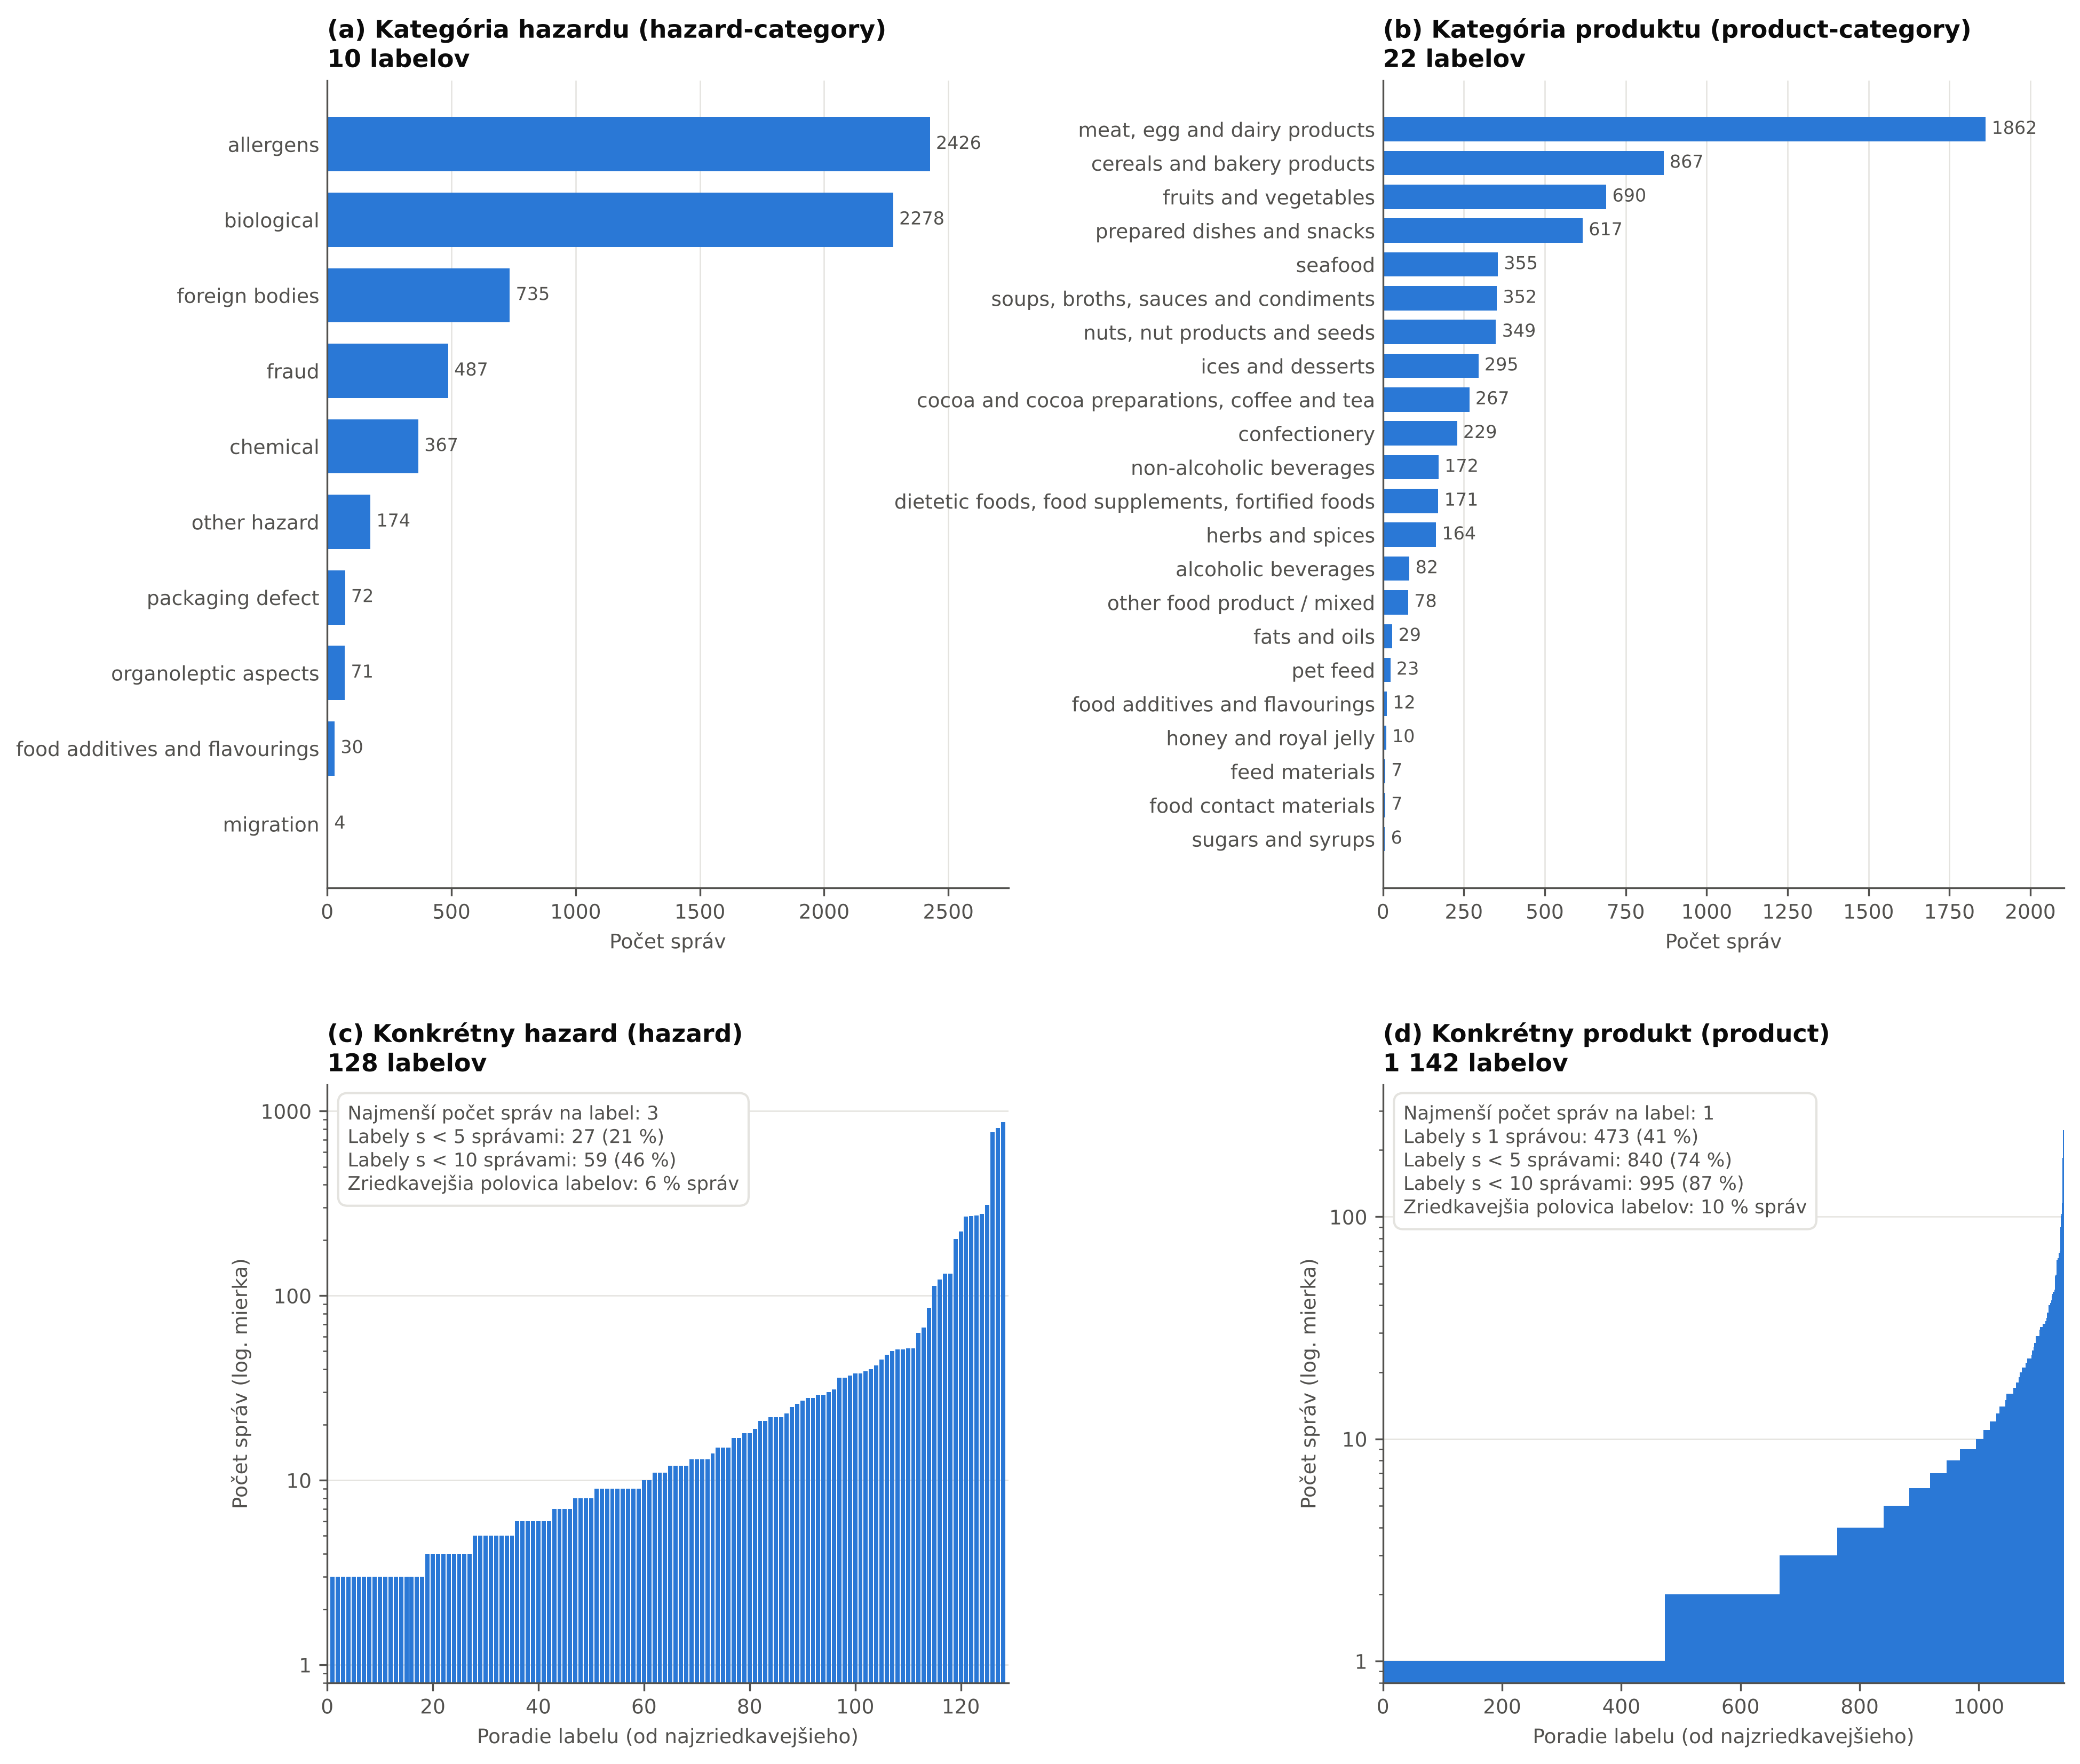
\includegraphics[width=0.95\textwidth]{figures/dataset_distribution.png}
    \caption{Distribúcie cieľových atribút v poskytnutom datasete.}
    \label{fig:dataset_distribution}
\end{figure}

\begin{comment}
\subsection{Prehľad riešení dosahujúcich najlepšie výsledky}

The most important literature source for this project is the official SemEval-2025 Task 9 report \cite{randl-etal-2025-semeval}. Included within this report is a section highlighting the 4 best performing submitted solutions with references to their individual papers. The following subsections will briefly describe the methods used in the solutions. This information will then be used in order to formulate an appropriate baseline for this project.

\subsubsection{SRCB (Ricoh Software Research Center (Beijing)) \cite{zhang-etal-2025-srcb}} 

For data pre-processing the system first concatenates the \textit{title} and \textit{text} (which were the only input features used) into a single text format, which is then cleaned to remove various text artifacts such as line breaks, spaces, duplicate lines etc. The resulting texts are then truncated to a maximum token length in order to be used for inputs for the two modules the system employs (512 and 1024 respectively).   

For data augmentation a method involving an LLM was used (specifically the Qwen2.5-72B-Instruct), where the LLM was instructed to create a new sample based on the meaning and label of a target sample from a rare (fewer than 50 occurrences in the training data) class and writing style and format of a randomly selected sample.

The actual system used two primary modules : a candidate recall module and an LLM prediction module. The role of the candidate recall module is to help narrow the set of possible output labels before the more computationally expensive LLM prediction. This module uses a one-vs-all approach, constructing a binary classifier for each label on top of a BERT architecture. This approach was chosen due to the fact that the authors experimented with the RoBERTa-base model and found that while the score for classification was rather poor, the recall score achieved a value over 95\% indicating that the correct label would almost always be found in the candidate labels outputted by the BERT model. In the final submission this module was built using the RoBERTa-base and DeBERTaV3-base models.

The LLM prediction module is more complex, involving two LLMs : a fine tuned target LLM and a frozen reference LLM that is used to pre-compute embeddings of all labels before training. These embeddings are then used as external background knowledge together with the output of the target LLM (which uses the formatted text body and the reduced label set from the previous module) inside of a multi-head attention module, the outputs of which are then used to generate the final label as text. For both roles the authors used the Qwen2.5-14B-Base model. The final submission from this team combined several variants of this pipeline with majority voting, however the exact details of the variants used are not described in the report. 

This solution ranked third for ST1 and first(!) for ST2, with two separate but architecturally same pipelines for each subtask. 

\begin{figure}
    \centering
    \includegraphics[width=0.95\textwidth]{figures/SRCB_Figure2_LLM_Prediction_Module.png}
    \caption{Architecture of the LLM prediction module (taken directly from \cite{zhang-etal-2025-srcb}).}
    \label{fig:srcb_llm_prediction_module}
\end{figure}
\end{comment}

\subsection{Prehľad riešení dosahujúcich najlepšie výsledky}

Najdôležitejším literárnym zdrojom pre tento projekt je oficiálna správa k SemEval-2025 Task 9 \cite{randl-etal-2025-semeval}. Táto správa obsahuje sekciu, v ktorej sú vyzdvihnuté 4 najlepšie odovzdané riešenia spolu s odkazmi na ich jednotlivé články. V nasledujúcich podkapitolách budú stručne opísané metódy použité v týchto riešeniach. Tieto informácie budú následne použité na sformulovanie vhodného baseline riešenia pre tento projekt.

\subsubsection{SRCB (Ricoh Software Research Center (Beijing)) \cite{zhang-etal-2025-srcb}}

V rámci predspracovania dát systém najprv spojí atribúty \textit{title} a \textit{text} (ktoré boli jedinými použitými vstupnými atribútmi) do jedného textu, ktorý je následne vyčistený od rôznych textových artefaktov, ako sú zalomenia riadkov, nadbytočné medzery, duplicitné riadky a pod. Výsledné texty sú následne skrátené na maximálnu dĺžku v tokenoch, aby mohli byť použité ako vstupy pre dva moduly, ktoré systém využíva (512, resp. 1024 tokenov).

Na augmentáciu dát bola použitá metóda využívajúca LLM (konkrétne model Qwen2.5-72B-Instruct), pričom LLM bol inštruovaný vytvoriť novú vzorku, ktorá preberá význam a označenie cieľovej vzorky zo zriedkavej triedy (menej ako 50 výskytov v trénovacích dátach) a štýl písania a formát náhodne vybranej vzorky.

Samotný systém využíval dva hlavné moduly: modul na výber kandidátov (candidate recall module) a modul predikcie pomocou LLM (LLM prediction module). Úlohou modulu na výber kandidátov je zúžiť množinu možných výstupných označení pred výpočtovo náročnejšou predikciou pomocou LLM. Tento modul využíva prístup one-vs-all, pričom pre každé označenie je zostrojený binárny klasifikátor nad architektúrou BERT. Tento prístup bol zvolený, pretože autori experimentovali s modelom RoBERTa-base a zistili, že hoci skóre klasifikácie bolo pomerne slabé, hodnota recall presahovala 95~\%, čo naznačuje, že správne označenie sa takmer vždy nachádza medzi kandidátskymi označeniami na výstupe modelu BERT. Vo finálnom odovzdanom riešení bol tento modul zostavený s použitím modelov RoBERTa-base a DeBERTaV3-base.

Modul predikcie pomocou LLM je zložitejší a zahŕňa dva LLM: doladený (fine-tuned) cieľový LLM a zmrazený referenčný LLM, ktorý je použitý na predvýpočet embeddingov všetkých označení ešte pred trénovaním. Tieto embeddingy sú následne použité ako externé doplnkové znalosti spolu s výstupom cieľového LLM (ktorý na vstupe dostáva naformátovaný text a zúženú množinu označení z predchádzajúceho modulu) v module multi-head attention, ktorého výstupy sú následne použité na vygenerovanie výsledného označenia vo forme textu. Pre obe roly autori použili model Qwen2.5-14B-Base. Finálne odovzdané riešenie tohto tímu kombinovalo niekoľko variantov tejto pipeline pomocou väčšinového hlasovania, avšak presné detaily použitých variantov nie sú v správe opísané.

Toto riešenie sa umiestnilo na treťom mieste v ST1 a na prvom(!) mieste v ST2, pričom pre každú podúlohu bola použitá samostatná, no architektonicky rovnaká pipeline.

\begin{figure}
    \centering
    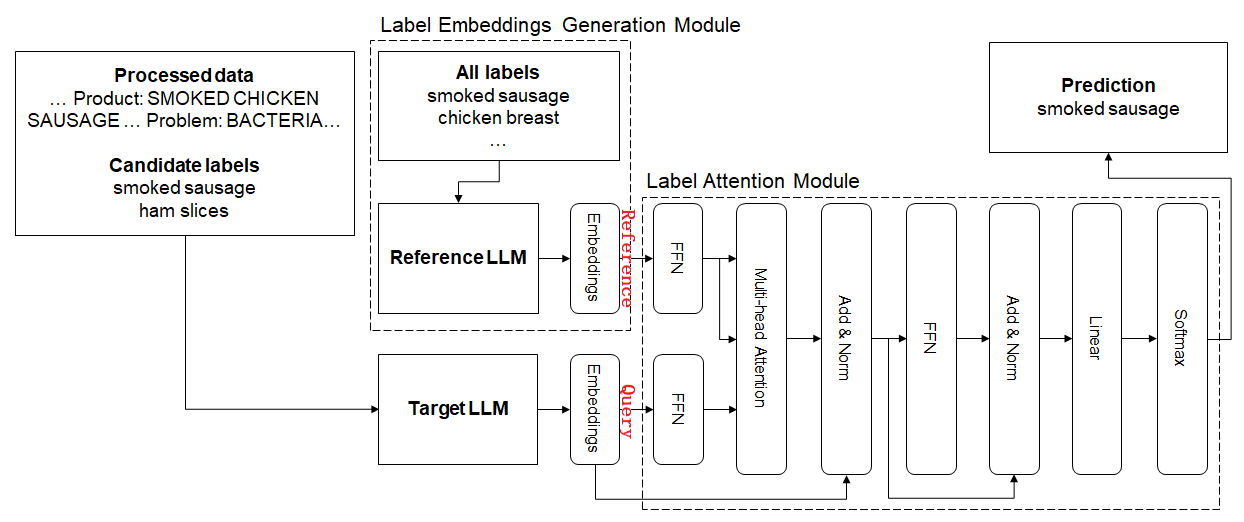
\includegraphics[width=0.95\textwidth]{figures/srcb_prediction_module.png}
    \caption{Architektúra modulu predikcie pomocou LLM (prevzaté priamo z \cite{zhang-etal-2025-srcb}).}
    \label{fig:srcb_llm_prediction_module}
\end{figure}

\begin{comment}
\subsubsection{Anastasia \cite{le-etal-2025-anastasia}}

This system uses an ensemble approach focusing exclusively on ST1. For data pre-processing the system first (seemingly) concatenates all of the provided input features.Standard text cleaning techniques are then applied to remove artifacts similar to the SRCB solution. Various degrees of data augmentation (including none) are then employed to create three separate datasets that are used by the system's modules. The resulting entries of the datasets are then divided into sentence-based chunks of various sizes in order to be used as inputs for the various models inside the modules, concretely sizes of 512, 768, 1024 and 1280 token chunks.

The three datasets used were:

\begin{enumerate}
    \item \textit{Original} -- features no synthetic samples, only oversampling and undersampling techniques, which were employed in order to help balance out the dataset
    
    \item \textit{Light Augmentation} -- features data augmentation, specifically the creation of synthetic samples of underpopulated classes (the exact method of the creation of these samples is not detailed in the article)
    
    \item \textit{Heavy Augmentation} -- same as Light Augmentation, however with larger quantities of synthetic samples and extra processing steps
\end{enumerate}

For the \textit{Heavy Augmentation} additional processing techniques were used such as HTML tag removal with the help of BeautifulSoup \cite{pant2024web} and the translation of the non-English entries included in the original data, helping to further increase the consistency and size of this variation of the dataset. 

As previously mentioned this solution uses three system modules, with two of these modules focusing on a single-task prediction (product category and hazard category respectively) and the third one on a multi-task prediction of both target features. The single-task modules in total feature 24 models (12 configurations for hazard and product category respectively) based on the combination of the light/heavy dataset, DeBERTa-v3-large/RoBERTa-large model, and the 512/768/1024/1280 token chunk size. For the multitask module only the DeBERTa-v3-large model was used with a token chunk size of 512, using the \textit{Original} dataset. For the exact combinations used see Figure~\ref{fig:anastasia_models}.

\begin{figure}
    \centering
    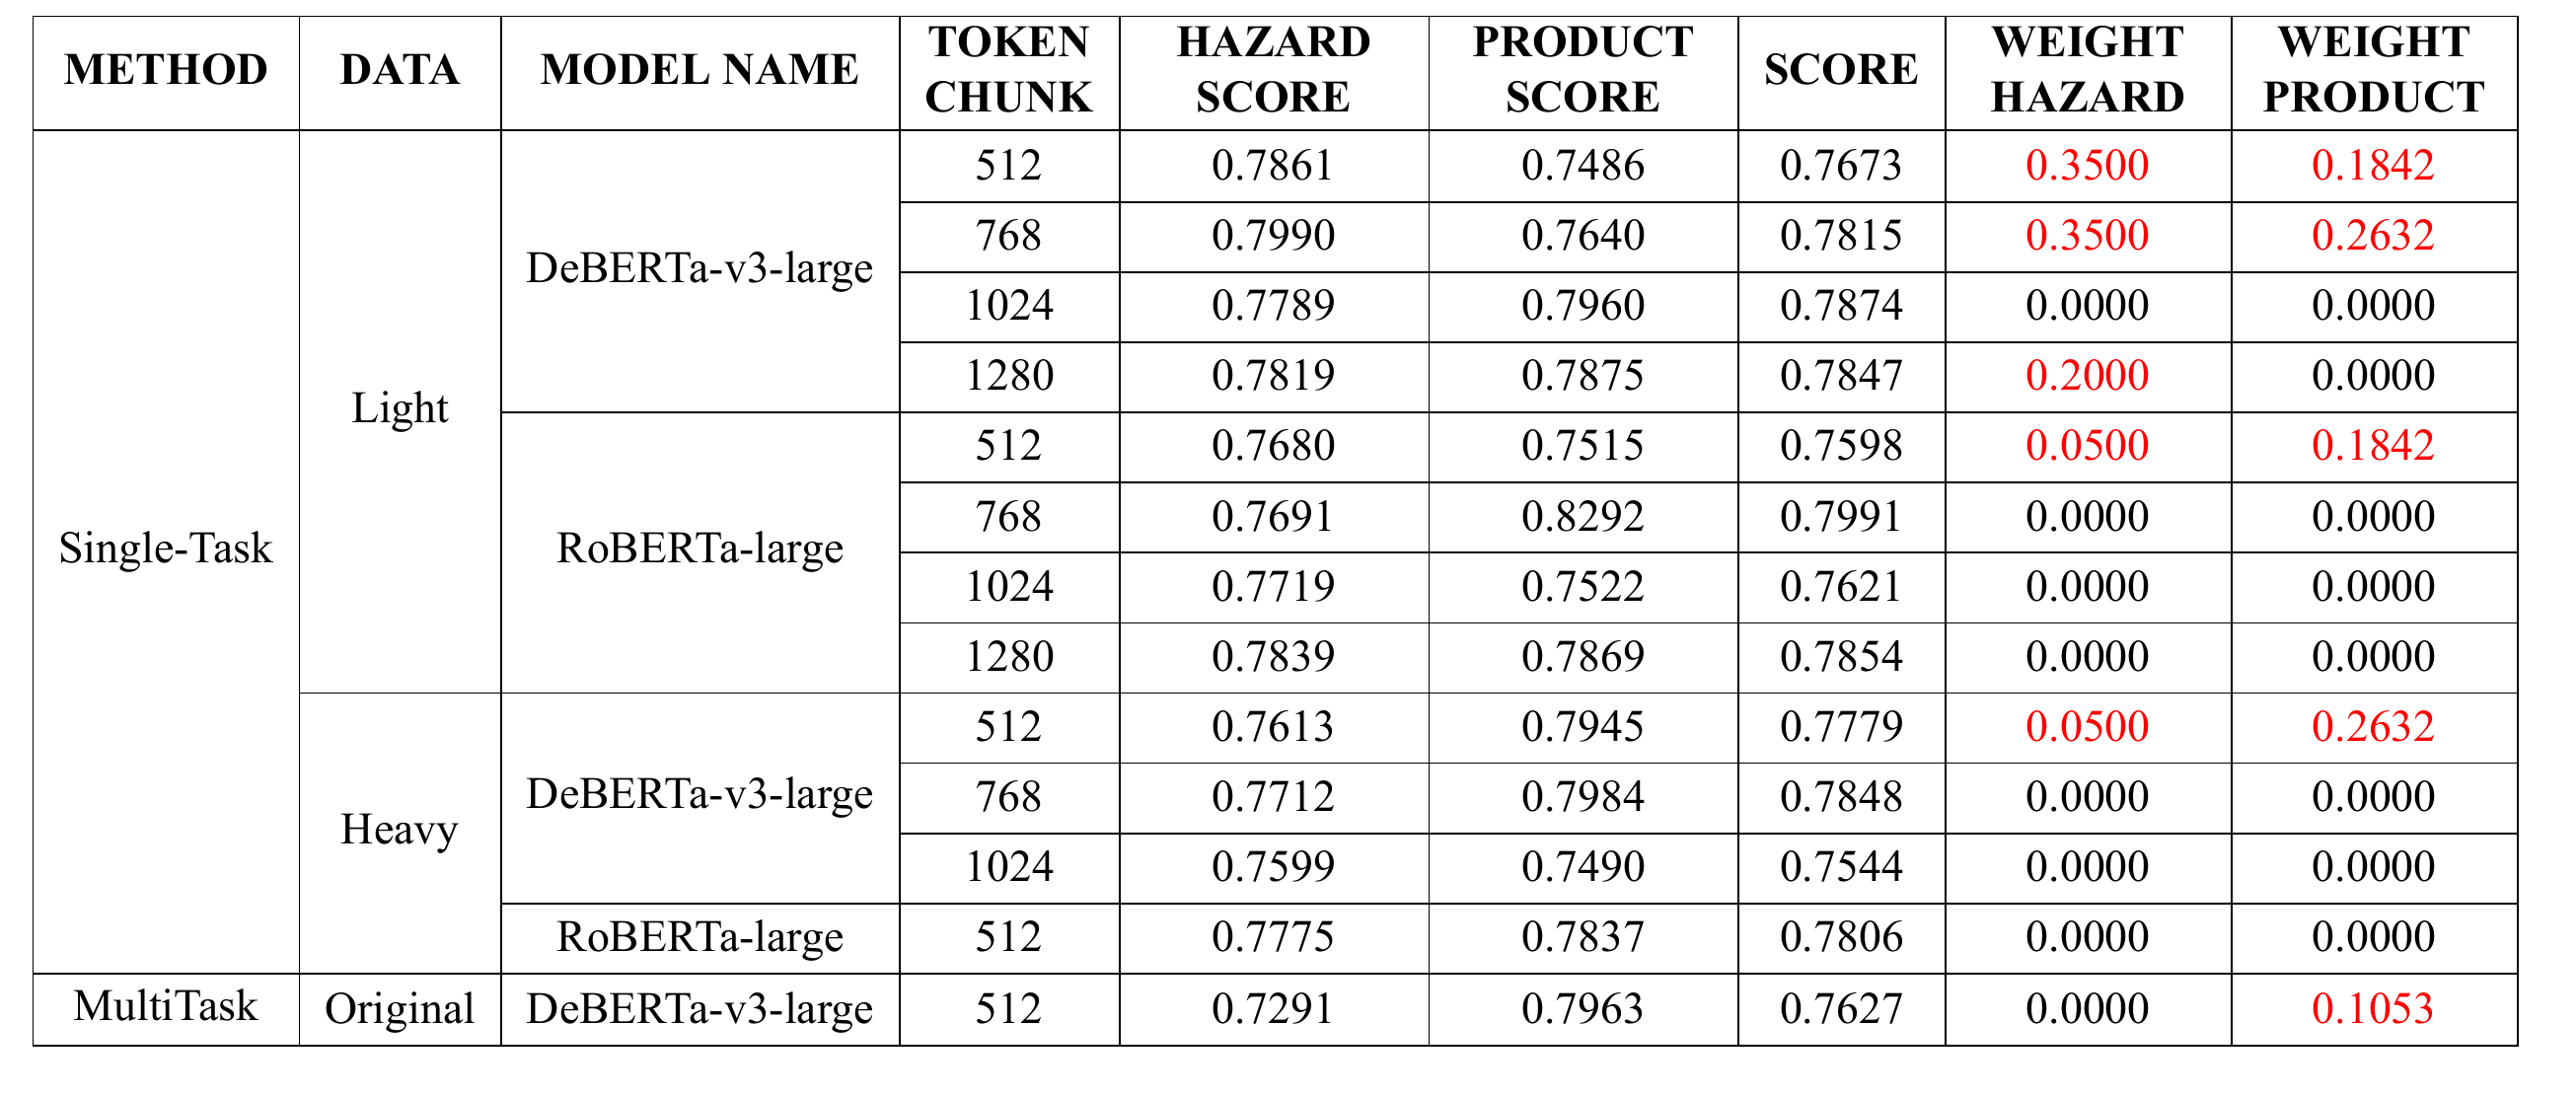
\includegraphics[width=0.95\textwidth]{figures/anastasia_models.png}
    \caption{Exact combinations of models used as part of the solution, each single-task row represents two models (one for the hazard and product category respectively) also including the final weights used in soft-voting (taken directly from \cite{le-etal-2025-anastasia}).}
    \label{fig:anastasia_models}
\end{figure}

To obtain the final prediction, weighted soft voting is applied separately for the hazard and product category, the exact weights of which were obtained with the help of a grid search technique. Another aspect that is important to highlight is the use of the loss function: Focal loss \cite{lin2017focal}. This loss function (see Equation~\eqref{eq:focal_loss}) is designed to reduce the impact of easy-to-classify samples  while prioritizing the harder ones, further helping to reduce the impact of the imbalanced dataset. This function was used in the fine-tuning process of all the models.

\begin{equation}
  \mathcal{L}_{FL}(p_t) = -\alpha_t (1 - p_t)^{\gamma} \log(p_t)
  \label{eq:focal_loss}
\end{equation}

This solution ranked first(!) for ST1. However, the authors acknowledge that they submitted multiple test runs, violating SemEval's single-submission rule, which may have given them an advantage.
\end{comment}

\subsubsection{Anastasia \cite{le-etal-2025-anastasia}}

Tento systém využíva ensemble prístup a zameriava sa výlučne na ST1. V rámci predspracovania dát systém najprv (zrejme) spojí všetky poskytnuté vstupné atribúty. Následne sú aplikované štandardné techniky čistenia textu na odstránenie artefaktov, podobne ako v riešení SRCB. Potom je použitá augmentácia dát v rôznej miere (vrátane žiadnej) na vytvorenie troch samostatných datasetov, ktoré sú využívané modulmi systému. Záznamy výsledných datasetov sú následne rozdelené na úseky (chunky) založené na vetách s rôznou veľkosťou, aby mohli byť použité ako vstupy pre jednotlivé modely v moduloch, konkrétne s veľkosťou 512, 768, 1024 a 1280 tokenov.

Použité boli tieto tri datasety:

\begin{enumerate}
    \item \textit{Original} -- neobsahuje syntetické vzorky, iba techniky oversamplingu a undersamplingu, ktoré boli použité na vyváženie datasetu
    
    \item \textit{Light Augmentation} -- obsahuje augmentované dáta, konkrétne syntetické vzorky málo zastúpených tried (presná metóda vytvorenia týchto vzoriek nie je v článku opísaná)
    
    \item \textit{Heavy Augmentation} -- rovnaký ako Light Augmentation, avšak s väčším množstvom syntetických vzoriek a dodatočnými krokmi spracovania
\end{enumerate}

Pri datasete \textit{Heavy Augmentation} boli použité dodatočné techniky spracovania, ako napríklad odstránenie HTML tagov pomocou knižnice BeautifulSoup \cite{pant2024web} a preklad neanglických záznamov obsiahnutých v pôvodných dátach, čo pomohlo ďalej zvýšiť konzistenciu a veľkosť tejto verzie datasetu.

Ako už bolo spomenuté, toto riešenie využíva tri moduly, pričom dva z nich sa zameriavajú na predikciu jedného cieľového atribútu (single-task), konkrétne kategórie produktu, resp. kategórie hazardu, a tretí na súčasnú predikciu oboch cieľových atribútov (multi-task). Single-task moduly spolu obsahujú 24 modelov (12 konfigurácií pre kategóriu hazardu a 12 pre kategóriu produktu), ktoré vychádzajú z kombinácie datasetu light/heavy, modelu DeBERTa-v3-large/RoBERTa-large a veľkosti chunku 512/768/1024/1280 tokenov. Pre multi-task modul bol použitý iba model DeBERTa-v3-large s veľkosťou chunku 512 tokenov a datasetom \textit{Original}. Pre použité kombinácie viď obrázok~\ref{fig:anastasia_models}.

\begin{figure}
    \centering
    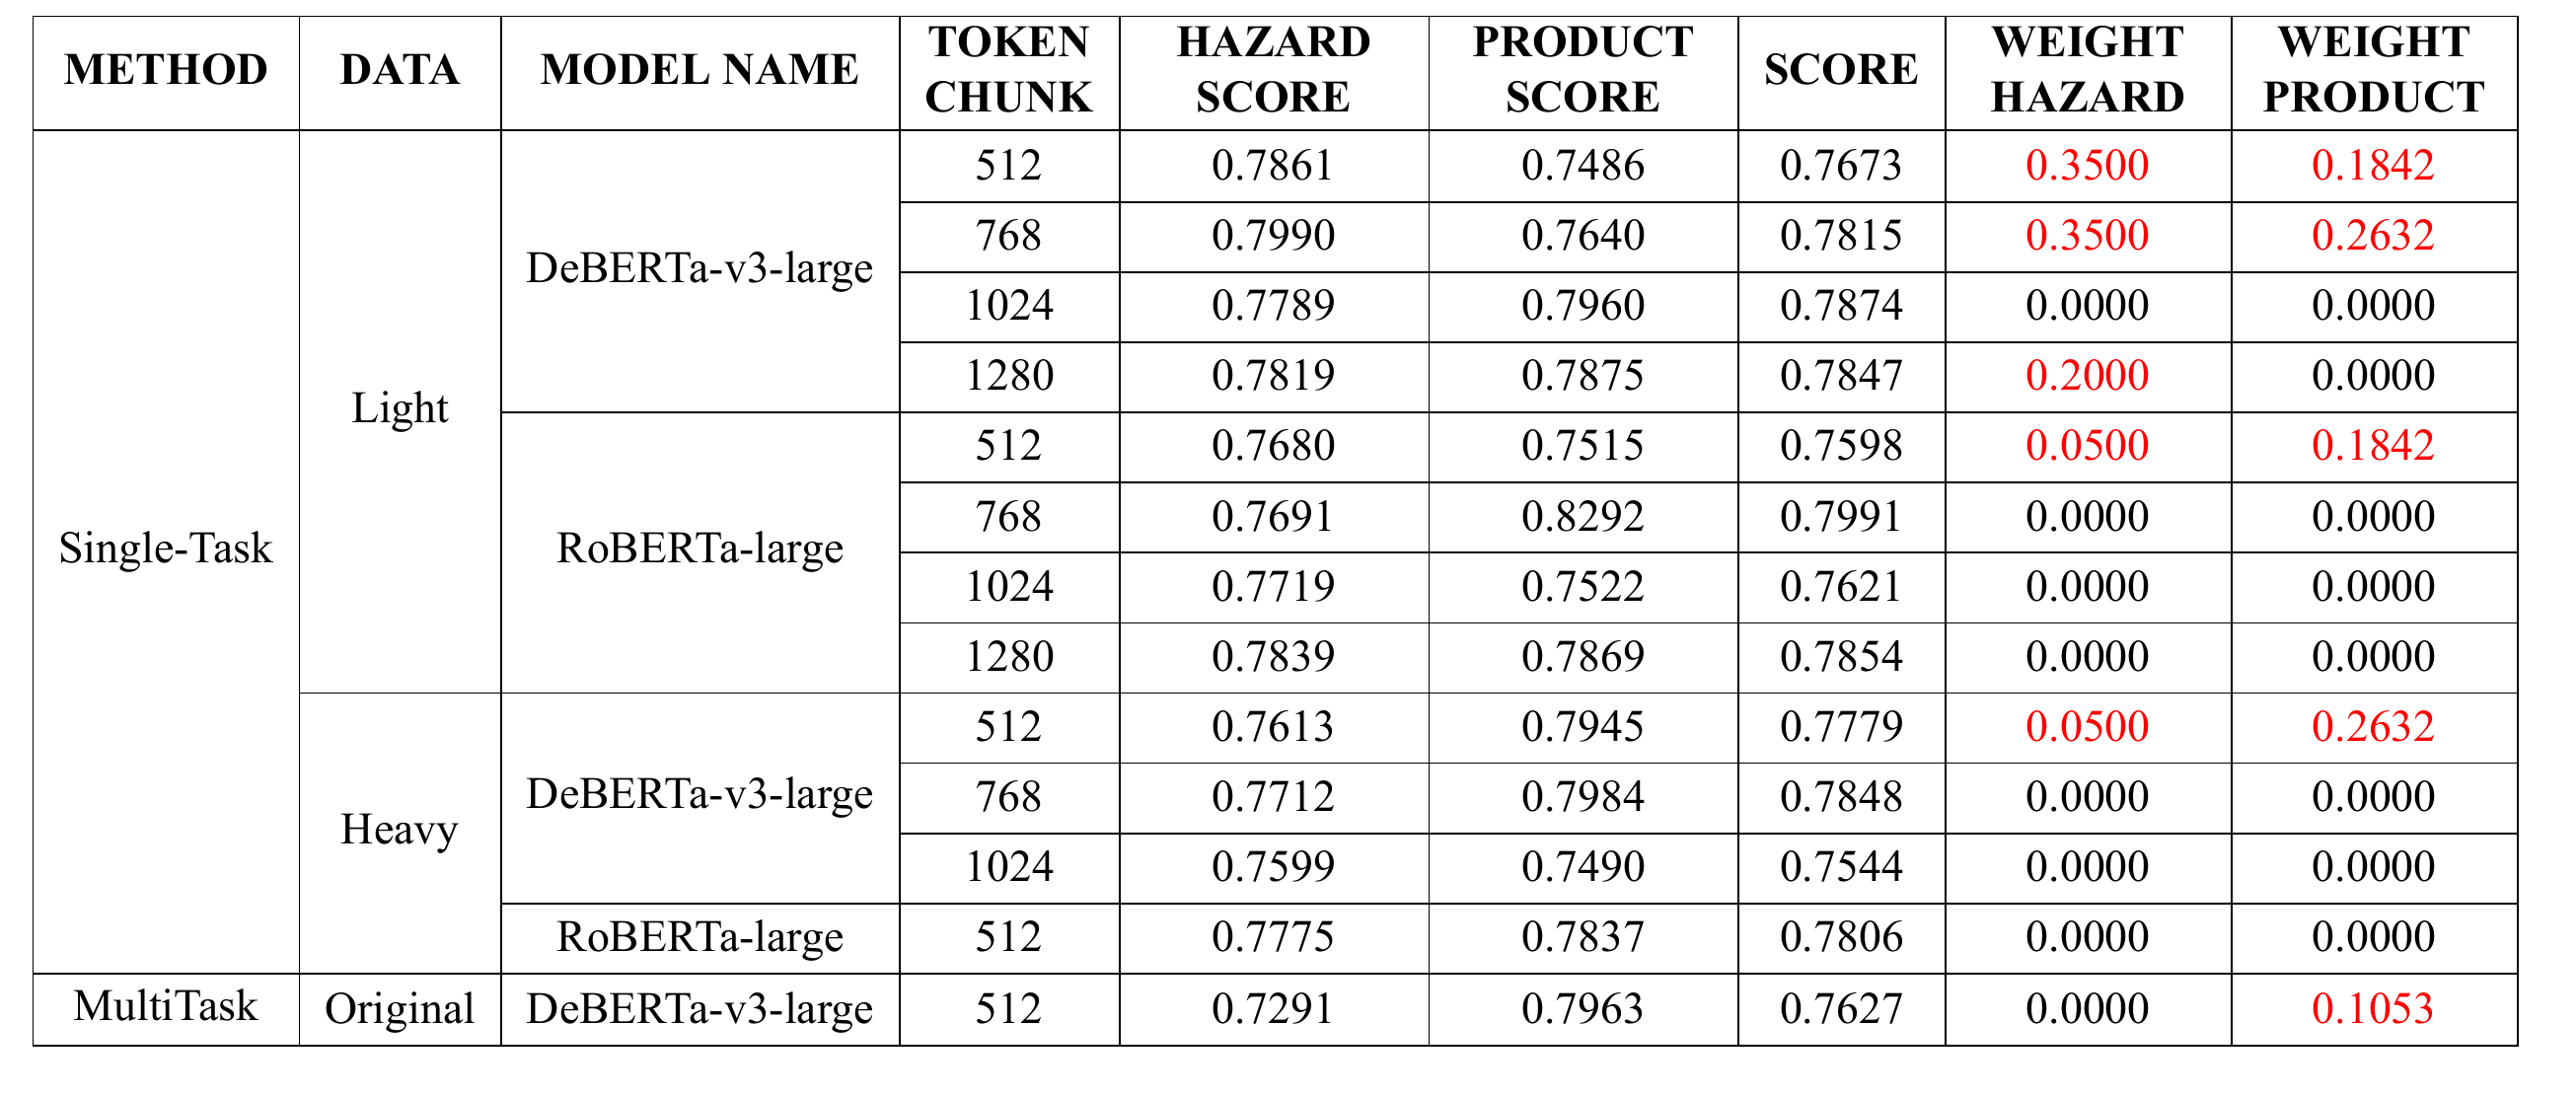
\includegraphics[width=0.95\textwidth]{figures/anastasia_models.png}
    \caption{Presné kombinácie modelov použitých v riešení. Každý single-task riadok predstavuje dva modely (jeden pre kategóriu hazardu a jeden pre kategóriu produktu) a obsahuje aj výsledné váhy použité pri mäkkom hlasovaní (prevzaté priamo z \cite{le-etal-2025-anastasia}).}
    \label{fig:anastasia_models}
\end{figure}

Na získanie finálnej predikcie je samostatne pre kategóriu hazardu a kategóriu produktu použité vážené mäkké hlasovanie (weighted soft voting), pričom presné váhy boli získané pomocou techniky grid search. Ďalším dôležitým aspektom, ktorý je potrebné zdôrazniť, je použitie loss funkcie Focal loss \cite{lin2017focal}. Táto loss funkcia (viď rovnicu~\eqref{eq:focal_loss}) je navrhnutá tak, aby znižovala vplyv ľahko klasifikovateľných vzoriek a uprednostňovala tie ťažšie, čo ďalej pomáha zmierniť vplyv nevyváženosti datasetu. Táto funkcia bola použitá pri doladení (fine-tuning) všetkých modelov.

\begin{equation}
  \mathcal{L}_{FL}(p_t) = -\alpha_t (1 - p_t)^{\gamma} \log(p_t)
  \label{eq:focal_loss}
\end{equation}

Toto riešenie sa umiestnilo na prvom(!) mieste v ST1. Autori však uvádzajú, že odovzdali viacero testovacích behov, čím porušili pravidlo SemEval o jedinom odovzdaní, čo im mohlo poskytnúť výhodu.

\begin{comment}
\subsubsection{MyMy \cite{phan-chiang-2025-mymy}}

This system is notable due to its focus on creating robust synthetic samples as part of data augmentation. For pre-processing the system does not seem to employ any sort of standard text cleaning procedure, only stating that the solution utilizes all provided input features.

The most important component of this system is the robust data augmentation pipeline, which utilizes a RAG technique in order to create rich synthetic samples to add to the dataset based on contextual documents retrieved from PubMed, a publicly accessible database for biomedical literature. First the original samples are fed to LLMs which are prompted with creating a short search query for each sample. This is done to help increase the effectiveness of document retrieval from PubMed API, which is otherwise prone to failure with complex queries. Based on the query the relevant documents are then retrieved from the PubMed API, and subsequently converted into dense vectors and stored in a Chroma vector database for efficient searching by cosine similarity. Next, the top-K (the value of this parameter is not stated in the report) most similar documents to the original text are inserted (together with original text itself) into the prompt format of the following step.

The resulting prompts are then passed to LLMs, which are instructed (as part of the prompt) with creating a synthetic sample by paraphrasing the original text while using the provided context. As a final step of data augmentation the resulting texts are then passed to LLMs, which are prompted with grading the quality of the created sample with a score from 0 to 5, based on relevance and accuracy against the included context. Only samples that receive a score of 4 or 5 are added to the resulting dataset. Roughly 60\,000 augmented samples passed this filtering step and were added to the dataset against the 5\,082 original samples, helping greatly in increasing the size of the dataset. The LLMs used in this augmentation pipeline were GPT-3.5 Turbo, Gemini Flash 2.0, Llama 3.1 8B, and Mixtral 8x7B. 

Compared to the data augmentation pipeline, the prediction pipeline is rather simple utilizing Gemini Flash 2.0, PubMedBERT and ModernBERT fine-tuned on the enriched dataset. The predicted labels are then computed using an ensemble strategy, specifically by averaging class probabilities of each of the models for each sub-task.

This solution ranked second on both ST1 and ST2, demonstrating itself as the most balanced of the highlighted solutions.  

\begin{figure}
    \centering
    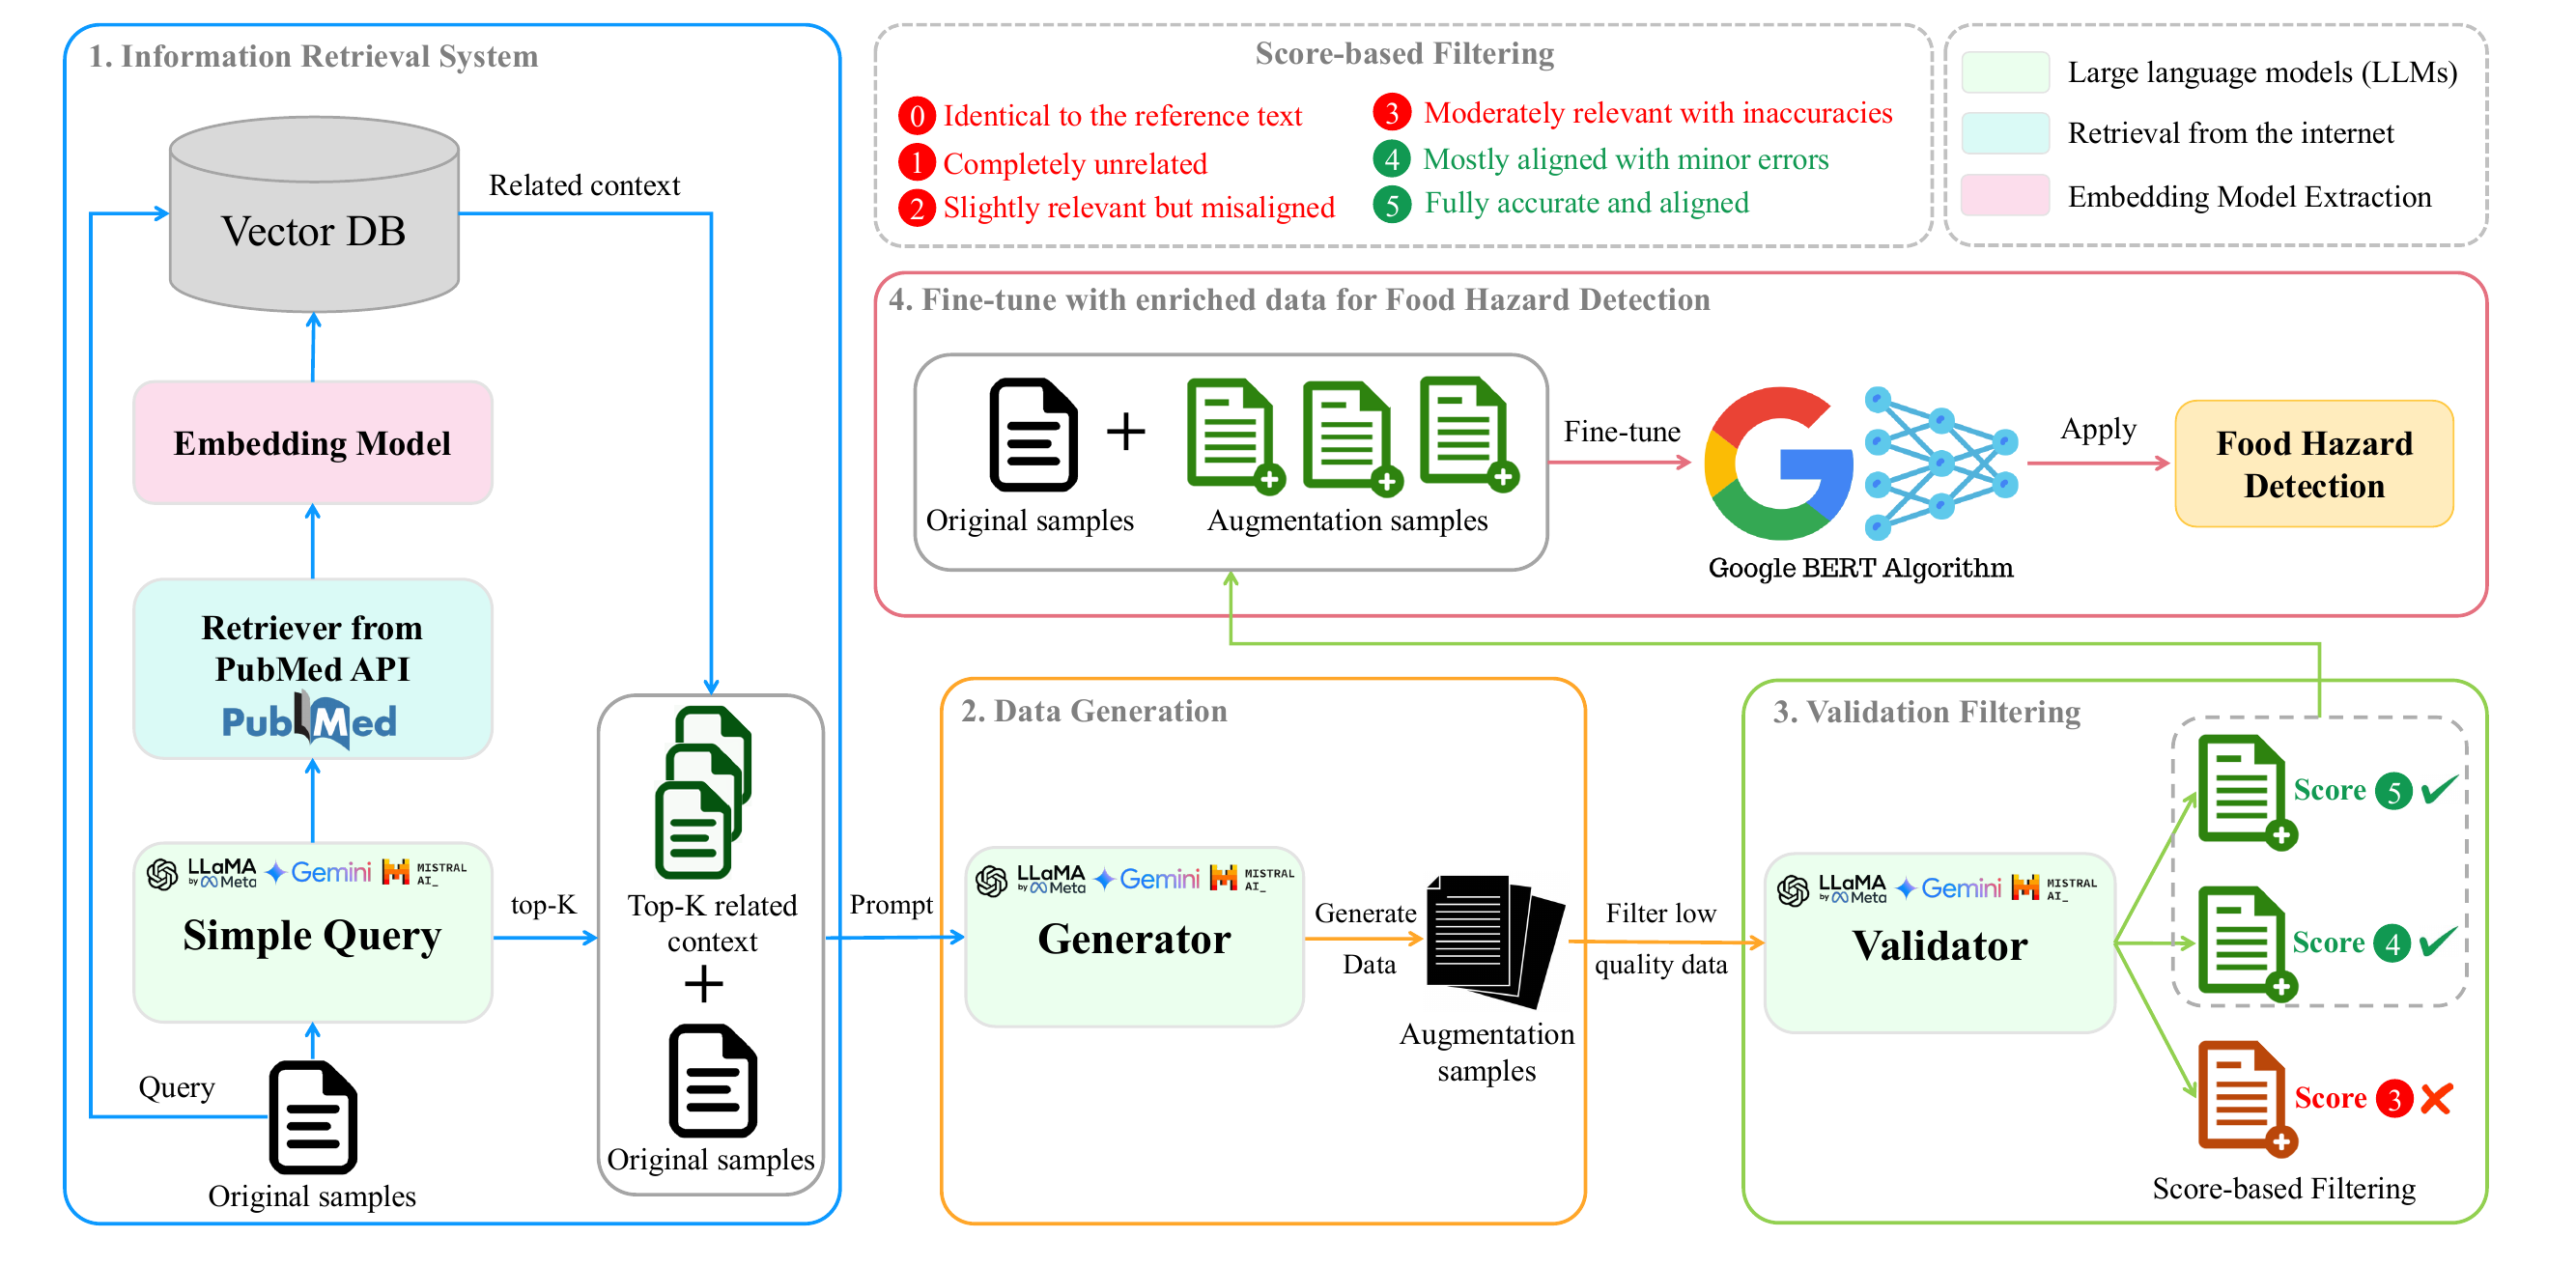
\includegraphics[width=0.95\textwidth]{figures/mymy_architecture.png}
    \caption{Data augmentation pipeline and system architecture used in the MyMy solution, Google BERT is only used as a visualization, the models fine-tuned as a part of the solution were Gemini Flash 2.0, PubMedBERT
    and ModernBERT (taken directly from \cite{phan-chiang-2025-mymy}).}
    \label{fig:mymy_architecture}
\end{figure}
\end{comment}

\subsubsection{MyMy \cite{phan-chiang-2025-mymy}}

Tento systém je pozoruhodný vďaka zameraniu na tvorbu robustných syntetických vzoriek v rámci augmentácie dát. V rámci predspracovania systém zrejme nevyužíva žiadny štandardný postup čistenia textu, pričom autori uvádzajú iba to, že riešenie využíva všetky poskytnuté vstupné atribúty.

Najdôležitejšou súčasťou tohto systému je robustná pipeline na augmentáciu dát, ktorá využíva techniku RAG na tvorbu obsahovo bohatých syntetických vzoriek pridávaných do datasetu na základe kontextových dokumentov získaných z PubMed, verejne dostupnej databázy biomedicínskej literatúry. Najprv sú pôvodné vzorky predané LLM, ktoré sú inštruované vytvoriť pre každú vzorku krátky vyhľadávací dopyt. Účelom tohto kroku je zvýšiť efektivitu získavania dokumentov z PubMed API, ktoré je inak pri zložitých dopytoch náchylné na zlyhanie. Na základe dopytu sú následne z PubMed API získané relevantné dokumenty, ktoré sú potom prevedené na dense vektory a uložené vo vektorovej databáze Chroma na efektívne vyhľadávanie pomocou kosínusovej podobnosti. Ďalej je top-K dokumentov najpodobnejších pôvodnému textu (hodnota tohto parametra nie je v správe uvedená) vložených (spolu so samotným pôvodným textom) do promptu nasledujúceho kroku.

Výsledné prompty sú následne predané LLM, ktoré sú (v rámci promptu) inštruované vytvoriť syntetickú vzorku parafrázovaním pôvodného textu s využitím poskytnutého kontextu. V poslednom kroku augmentácie dát sú výsledné texty predané LLM, ktoré sú inštruované ohodnotiť kvalitu vytvorenej vzorky od 0 do 5 na základe relevantnosti a presnosti vzhľadom na priložený kontext. Do výsledného datasetu sú pridané iba vzorky, ktoré získali skóre 4 alebo 5. Týmto filtrovaním úspešne prešlo približne 60\,000 augmentovaných vzoriek, ktoré boli pridané do datasetu oproti 5\,082 pôvodným vzorkám, čo výrazne pomohlo zväčšiť veľkosť datasetu. V tejto augmentačnej pipeline boli použité modely GPT-3.5 Turbo, Gemini Flash 2.0, Llama 3.1 8B a Mixtral 8x7B.

V porovnaní s pipeline na augmentáciu dát je predikčná pipeline pomerne jednoduchá a využíva modely Gemini Flash 2.0, PubMedBERT a ModernBERT doladené na obohatenom datasete. Predikované označenia sú následne vypočítané pomocou ensemble stratégie, konkrétne spriemerovaním pravdepodobností tried jednotlivých modelov pre každú podúlohu.

Toto riešenie sa umiestnilo na druhom mieste v ST1 aj ST2, čím sa ukázalo ako najvyváženejšie zo spomenutých riešení.

\begin{figure}
    \centering
    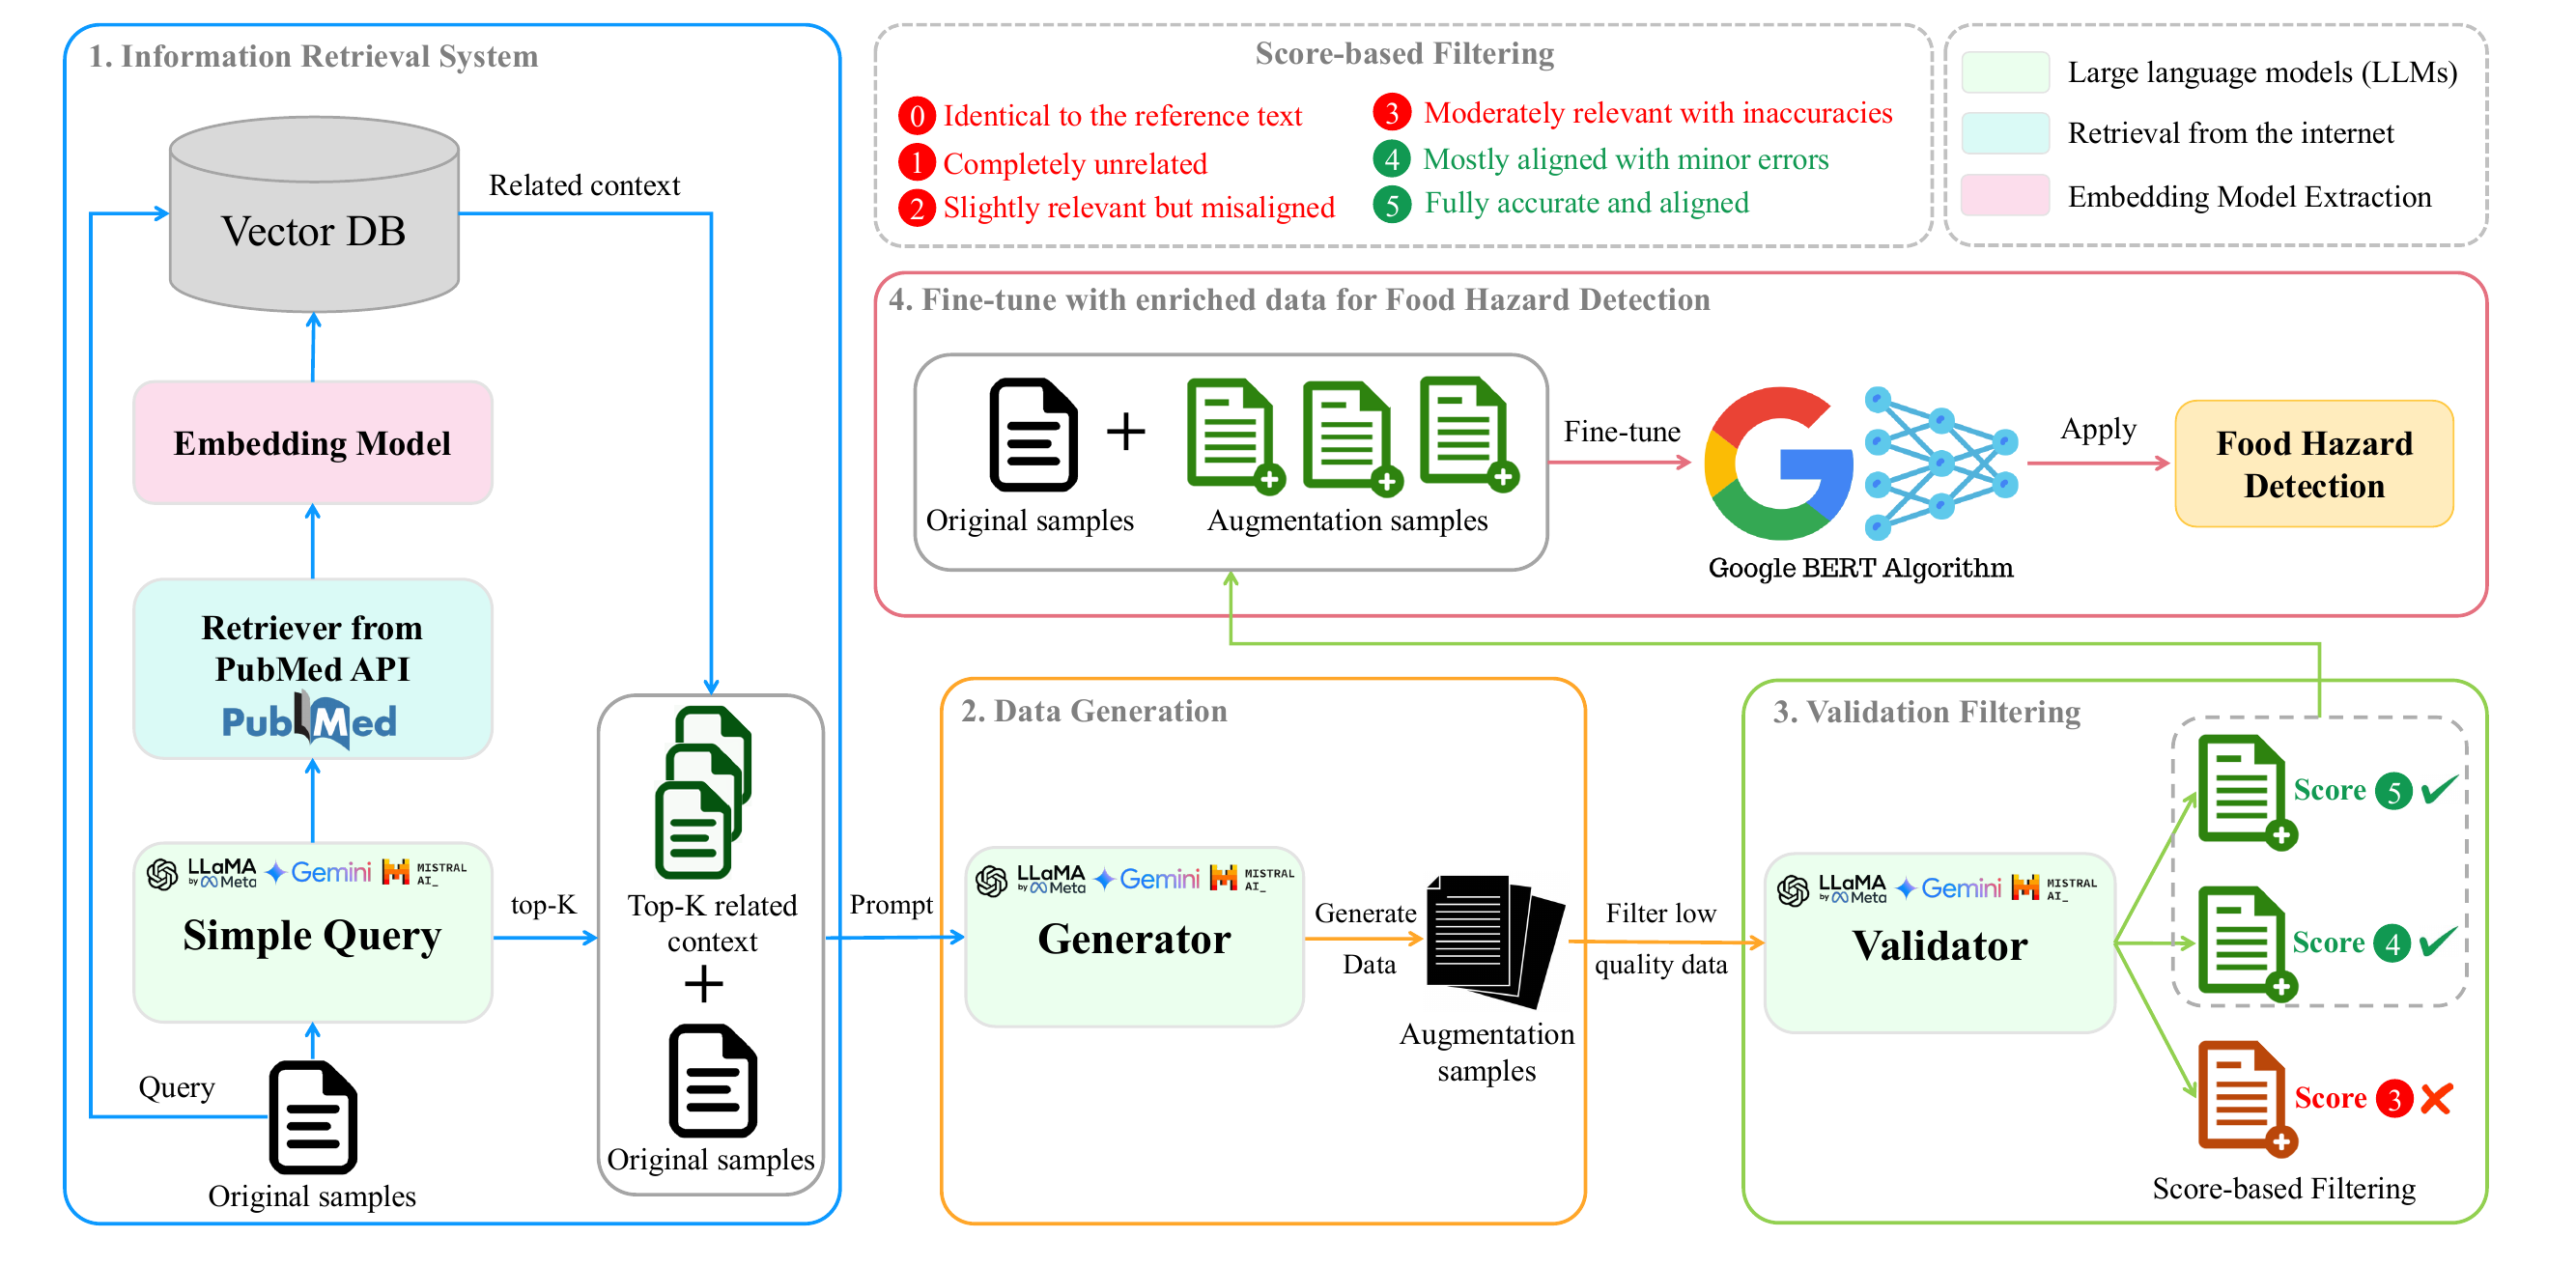
\includegraphics[width=0.95\textwidth]{figures/mymy_architecture.png}
    \caption{Pipeline na augmentáciu dát a architektúra systému použité v riešení MyMy. Google BERT slúži iba na ilustráciu, modely doladené v rámci riešenia boli Gemini Flash 2.0, PubMedBERT a ModernBERT (prevzaté priamo z \cite{phan-chiang-2025-mymy}).}
    \label{fig:mymy_architecture}
\end{figure}

\begin{comment}
\subsubsection{PATeam \cite{wan-etal-2025-pateam}}

This system is notable for its use of a single generative LLM that solves both sub-tasks jointly in a multi-turn dialogue format, combined with a bagging ensemble. For pre-processing, the authors use regular expressions to remove unwanted web artifacts such as hyperlinks, HTML formatting and e-mail addresses. Only the \textit{title} and \textit{text} input features are used.

For data augmentation, an LLM is prompted to generate a concise summary of each cleaned text, which is then concatenated with the original text. Unlike the other highlighted solutions, this does not create new samples but enriches the existing ones; according to the authors, the summaries help standardise the noisy texts and highlight the information relevant to the product and hazard labels. The LLM used for summarisation is not named in the text, although the system overview (Figure~\ref{fig:pateam_overview}) indicates Qwen2.5-72B. To address the class imbalance, the enriched dataset is then oversampled so that every class contains at least five samples, a threshold the authors found to work best on the validation set.

The prediction itself is done by Phi-4, fine-tuned with LoRA \cite{hu2021lora}, which formulates the two sub-tasks as a two-round dialogue. In the first round, the model receives the title, the cleaned text and the generated summary and predicts the hazard and product category (ST1). In the second round, these predictions are added to the prompt and the model is asked to infer the more specific hazard and product (ST2). This way, the coarse-grained prediction guides the fine-grained one. For the ensemble, a bagging approach \cite{breiman1996bagging} is used: five subsets of the training data are sampled with replacement, a separate Phi-4 model is fine-tuned on each of them, and the final prediction is obtained by voting between the five models (the exact voting scheme is not specified).

This solution ranked fourth in ST1 and third in ST2.

\begin{figure}
    \centering
    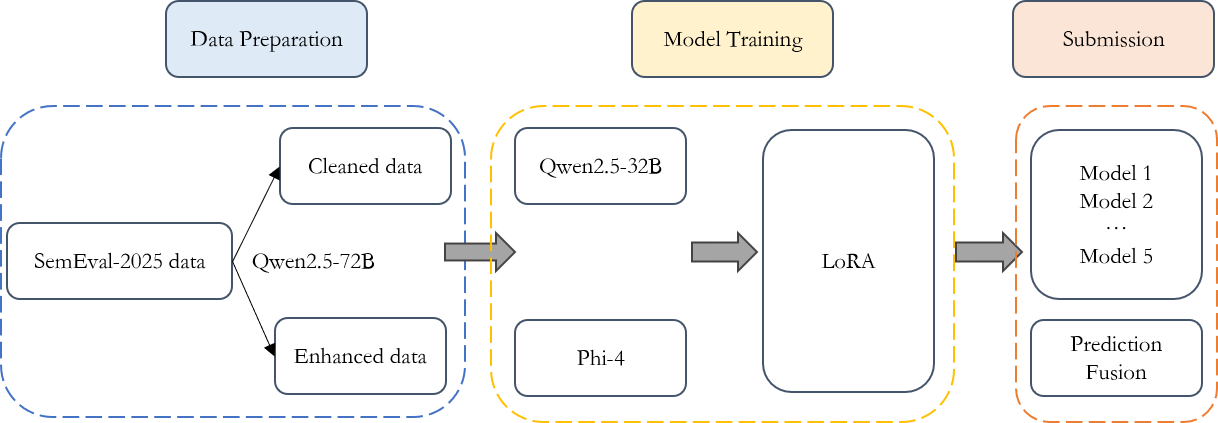
\includegraphics[width=0.95\textwidth]{figures/pateam_overview.png}
    \caption{System overview of the PATeam solution. Although Qwen2.5-32B is shown in the model training stage, all reported results were obtained with Phi-4 (taken directly from \cite{wan-etal-2025-pateam}).}
    \label{fig:pateam_overview}
\end{figure}
\end{comment}

\subsubsection{PATeam \cite{wan-etal-2025-pateam}}

Tento systém je pozoruhodný využitím jediného generatívneho LLM, ktorý rieši obe podúlohy spoločne vo forme viackolového dialógu, v kombinácii s bagging ensemble prístupom. V rámci predspracovania autori používajú regulárne výrazy na odstránenie nežiaducich webových artefaktov, ako sú hypertextové odkazy, HTML formátovanie a e-mailové adresy. Použité sú iba vstupné atribúty \textit{title} a \textit{text}.

V rámci augmentácie dát je LLM inštruovaný vygenerovať stručné zhrnutie každého vyčisteného textu, ktoré je následne spojené s pôvodným textom. Na rozdiel od ostatných spomenutých riešení tento prístup nevytvára nové vzorky, ale obohacuje existujúce. Podľa autorov zhrnutia pomáhajú štandardizovať zašumené texty a zvýrazniť informácie relevantné pre označenia produktu a hazardu. LLM použitý na tvorbu zhrnutí nie je v texte článku pomenovaný, avšak prehľad systému (obrázok~\ref{fig:pateam_overview}) naznačuje model Qwen2.5-72B. Na riešenie nevyváženosti tried je obohatený dataset následne oversamplovaný tak, aby každá trieda obsahovala aspoň päť vzoriek, pričom autori zistili, že táto hranica dosahuje na validačnej množine najlepšie výsledky.

Samotná predikcia je vykonávaná modelom Phi-4 doladeným pomocou LoRA \cite{hu2021lora}, ktorý formuluje obe podúlohy ako dialóg o dvoch kolách. V prvom kole model dostane nadpis, vyčistený text a vygenerované zhrnutie a predikuje kategóriu hazardu a kategóriu produktu (ST1). V druhom kole sú tieto predikcie pridané do promptu a model je požiadaný, aby určil konkrétnejší hazard a produkt (ST2). Týmto spôsobom všeobecnejšia predikcia usmerňuje tú detailnejšiu. Pre ensemble je použitý prístup bagging \cite{breiman1996bagging}: z trénovacích dát je vzorkovaním s opakovaním vytvorených päť podmnožín, na každej z nich je doladený samostatný model Phi-4 a finálna predikcia je získaná hlasovaním týchto piatich modelov (presná schéma hlasovania nie je uvedená).

Toto riešenie sa umiestnilo na štvrtom mieste v ST1 a na treťom mieste v ST2.

\begin{figure}
    \centering
    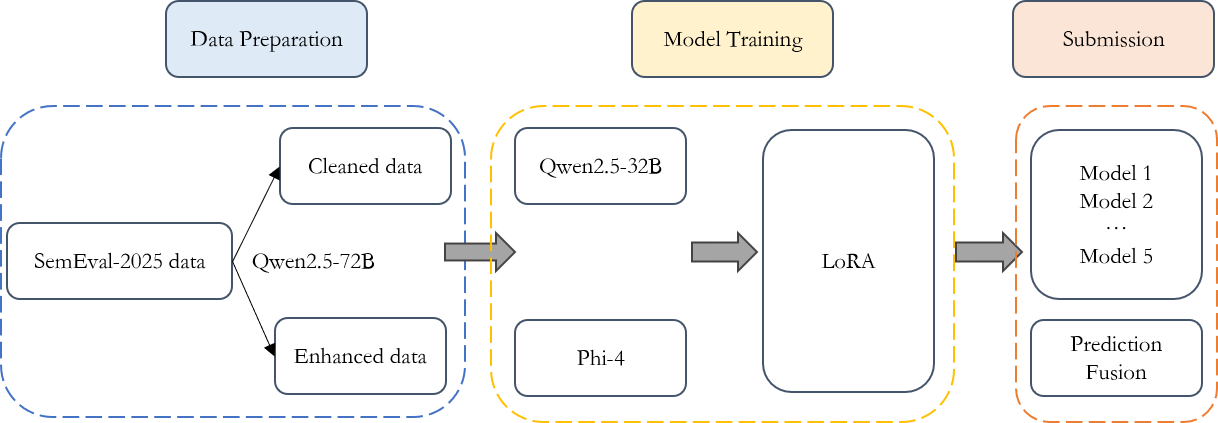
\includegraphics[width=0.95\textwidth]{figures/pateam_overview.png}
    \caption{Prehľad systému riešenia PATeam. Hoci je v štádiu trénovania modelu zobrazený model Qwen2.5-32B, všetky uvádzané výsledky boli získané s modelom Phi-4 (prevzaté priamo z \cite{wan-etal-2025-pateam}).}
    \label{fig:pateam_overview}
\end{figure}